%	The main skeletal structure
	\documentclass{standalone}
%	\def\pgfsysdriver{pgfsys-tex4ht.def}
%	\documentclass[twocolumn]{report}
	\usepackage{setspace}
	\usepackage{graphicx}
		\DeclareGraphicsExtensions{.pdf,.png,.eps,.ps}
	\usepackage{subcaption}
	\usepackage{lscape}
	\usepackage{pifont}
%	\usepackage{bbding}
	\usepackage{multirow}
	\usepackage{longtable}
	\usepackage[version=4]{mhchem}
	\usepackage{xfrac}
	\usepackage{color}
	\usepackage[colorlinks=true]{hyperref}
	\usepackage{gensymb}
	\usepackage{multicol}
		\setlength{\columnseprule}{0.4pt}
		\setlength{\columnsep}{5mm}
\makeatletter 
\newcounter{reaction} 
%%% >> for article << 
%\renewcommand\thereaction{C\,\arabic{reaction}} 
%%% << for article << 
%%% >> for report and book >> 
\renewcommand\thereaction{C\,\thechapter.\arabic{reaction}} 
\@addtoreset{reaction}{chapter} 
%%% << for report and book << 
\newcommand\reactiontag{\refstepcounter{reaction}\tag{\thereaction}} 
\newcommand\reaction@[2][]{\begin{equation}\ce{#2}% 
\ifx\@empty#1\@empty\else\label{#1}\fi% 
\reactiontag\end{equation}} 
\newcommand\reaction@nonumber[1]{\begin{equation*}\ce{#1}% 
\end{equation*}} 
\newcommand\reaction{\@ifstar{\reaction@nonumber}{\reaction@}} 
\makeatother 


	\usepackage[a4paper]{geometry}
	\usepackage{fullpage}
	\usepackage{fancyhdr}
%		\pagestyle{fancy}
%		\lhead{}
%		\chead{}
%		\rhead{\slshape \rightmark}
%		\fancyhead[LO,RE]{\slshape \leftmark} 
%		\fancyfoot[R]{\thepage} 
%	\renewcommand{\headrulewidth}{0.4pt} 
%	\renewcommand{\footrulewidth}{0.4pt} 
	\usepackage{cite}
	
%	\onehalfspacing
	\renewcommand{\baselinestretch}{1.5}
	
%	Footnote symbols
	\renewcommand{\thefootnote}{\fnsymbol{footnote}}

% Defining the chapter abstract area
%	\newenvironment{abstract}{\rightskip1in}{}

% Allow standard state notation
	\usepackage[varioref=false]{chemstyle}

% Allow for numbered examples
%	\usepackage{theorem,lipsum}
%	\theorembodyfont{\upshape}
%	\newtheorem{example}{Example}[chapter]
%	\newtheorem{question}{Question}[chapter]
%	\newtheorem{exercise}{Exercise}[chapter]
%	\newtheorem{concept}{Key Concept}[chapter]
%%%%%\begin{example}
%%%%%This is an example?
%%%%%\end{example}
%%%%%
%%%%%\begin{question}
%%%%%This is a quesiton?
%%%%%\end{question}

%%%%%FONT STUFF

%\usepackage[defaultfam,extralight,tabular,lining]{montserrat} %% Option 'defaultfam'
%%% only if the base font of the document is to be sans serif
%\usepackage[T1]{fontenc}
%\renewcommand*\oldstylenums[1]{{\fontfamily{Montserrat-TOsF}\selectfont #1}}

\usepackage{arev}
\usepackage[T1]{fontenc}
\usepackage{soul}

%%%%%TIKZ stuff
	\usepackage{tikz}
	\usepackage{pgfplots}
	\usetikzlibrary{decorations.pathmorphing,patterns,arrows,shapes.arrows}
	\usepgfplotslibrary{fillbetween}
	\tikzset{every picture/.style=remember picture}
		\newcommand{\mathnode}[1]{%
		\mathord{\tikz[baseline=(#1.base), inner sep = 0pt]{\node (#1) {$#1$};}}}

%%%%%% Grey stuff
%Need to define a shitload of greys...
\definecolor{gray1}{RGB}{240,240,240}
\definecolor{gray2}{RGB}{225,225,225}
\definecolor{gray3}{RGB}{210,210,210}
\definecolor{gray4}{RGB}{200,200,200}
\definecolor{gray5}{RGB}{180,180,180}


\begin{document}

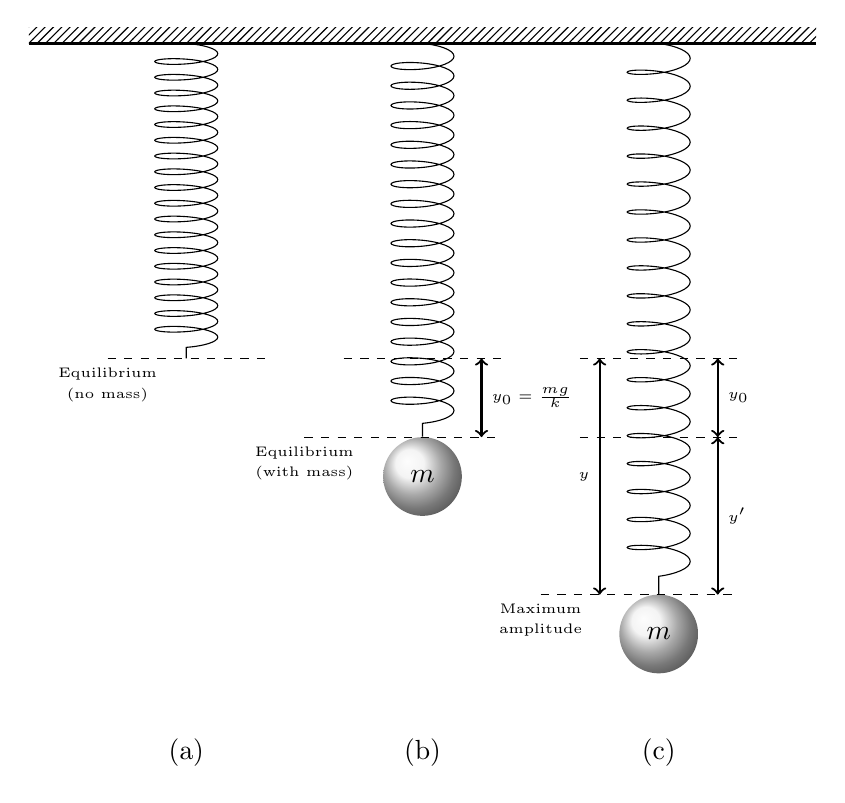
\begin{tikzpicture}[scale=1]
%\fill [pattern = north east lines] (-0.2,-0.8) rectangle (0,1);
\fill [pattern = north east lines] (0,0.2) rectangle (10,0);
%
%\draw[thick] (0,-0.6) -- (0,1);
\draw[thick] (0,0) -- (10,0);
%
\node[] (a1) at (2,0) {};
\node[] (b1) at (5,0) {};
\node[] (c1) at (8,0) {};
%
\node[] (a2) at (2,-4) {};
\node[circle,ball color=gray1,inner sep=0mm,minimum size=1cm] (b2) at (5,-5.5) {$m$};
\node[circle,ball color=gray1,inner sep=0mm,minimum size=1cm] (c2) at (8,-7.5) {$m$};
\draw[decoration={aspect=0.2, segment length=2mm, amplitude=4mm,coil},decorate] (2,0) -- (2,-4); 
\draw[decoration={aspect=0.25, segment length=2.5mm, amplitude=4mm,coil},decorate] (5,0) -- (b2); 
\draw[decoration={aspect=0.25, segment length=3.55mm, amplitude=4mm,coil},decorate] (8,0) -- (c2); 
%\draw[|-|,thick](0,-1)-- node[below] {$x_\textrm{0}$} (6,-1);
\draw[dashed] (1,-4)  -- (3,-4)  ;
\node[below] at (1,-4) {\tiny Equilibrium};
\node[below] at (1,-4.25) {\tiny (no mass)};
%
\draw[,dashed] (4,-4) node[below ]{}  -- (6,-4)  ;
%
\draw[,dashed] (3.5,-5) node[below ]{}  -- (6,-5)  ;
\node[below] at (3.5,-5) {\tiny Equilibrium};
\node[below] at (3.5,-5.25) {\tiny (with mass)};
%
\draw[,dashed] (7,-4) node[below ]{}  -- (9,-4)  ;
\draw[,dashed] (7,-5) node[below ]{}  -- (9,-5)  ;
\draw[,dashed] (6.5,-7) node[below ]{}  -- (9,-7)  ;
\node[below] at (6.5,-7) {\tiny Maximum};
\node[below] at (6.5,-7.25) {\tiny amplitude};
%
\node[]  at (2,-9) {(a)};
\node[]  at (5,-9) {(b)};
\node[]  at (8,-9) {(c)};
%
\draw[<->,thick] (5.75,-4) -- node[right]{\tiny $y_0 = \frac{mg}{k}$}(5.75,-5);
\draw[<->,thick] (7.25,-4) -- node[left]{\tiny $y$}(7.25,-7);
\draw[<->,thick] (8.75,-4) -- node[right]{\tiny $y_0$}(8.75,-5);
\draw[<->,thick] (8.75,-5) -- node[right]{\tiny $y'$}(8.75,-7);
%
%
%\draw[,dashed](8,-1.5)-- node[below] {} (8,0);
%\draw[<->,thick](6,-1)-- node[below] {$x$} (8,-1);
%
%\node[circle,ball color=gray,inner sep=5mm] (a) at (0,-2.5) {};
%\node[circle,ball color=gray,inner sep=5mm] (b) at (6,-2.5) {};
%\draw[decoration={aspect=0.2, segment length=3.04mm, amplitude=4mm,coil},decorate] (a) -- (b); 
%\draw[|-|,thick](0,-3.5)-- node[below] {$r_\textrm{0}$} (4.5,-3.5);
%\draw[<->|,thick](4.5,-3.5)-- node[below] {$R$} (6,-3.5);
%\draw[|<->|,thick](0,-4.5)-- node[below] {$r$} (6,-4.5);
\end{tikzpicture}

\end{document}

% Use the following to include the graphics in the chapter
%
%
%\begin{figure}[htbp]
%\begin{center}
%\includegraphics[scale=0.5]{images/fig-ch7_harmonicoscill0.pdf}
%\caption[Caption for list of figures]{Full caption to appear beside the image}
%\label{fig:label}
%\end{center}
%\end{figure}
 